\subsection{Xinanjiang model (model ID: 28)}
The Xinanjiang model (fig.~\ref{fig:28_schematic}) is originally intended for use in humid or semi-humid regions in China \citep{Zhao1992}. The model uses a variable contributing area to simulate runoff. The version presented here uses a double parabolic curve to simulate tension water capacities within the catchment \citep{Jayawardena2000}, instead of the original single parabolic curve. The model has 4 stores and 12 parameters ($A_{im}$, $a$, $b$, $W_{max}$, $LM$, $c$, $S_{max}$, $Ex$, $k_I$, $k_G$, $c_I$ and $c_G$). The model aims to represent:

\begin{itemizecompact}
\item Runoff from impervious areas;
\item Variable distribution of tension water storage capacities in the catchment;
\item Variable contributing area of free water storages;
\item Direct surface runoff from the contributing free area;
\item Delayed interflow and baseflow from the contributing free area.
\end{itemizecompact}

\subsubsection{File names}
\begin{tabular}{@{}ll}
Model: &m\_28\_xinanjiang\_12p\_4s \\
Parameter ranges: &m\_28\_xinanjiang\_12p\_4s\_parameter\_ ranges \\
\end{tabular}

% Equations
\subsubsection{Model equations}

% Model layout figure
{ 																	% This ensures it doesn't warp text further down
\begin{wrapfigure}{l}{6cm}
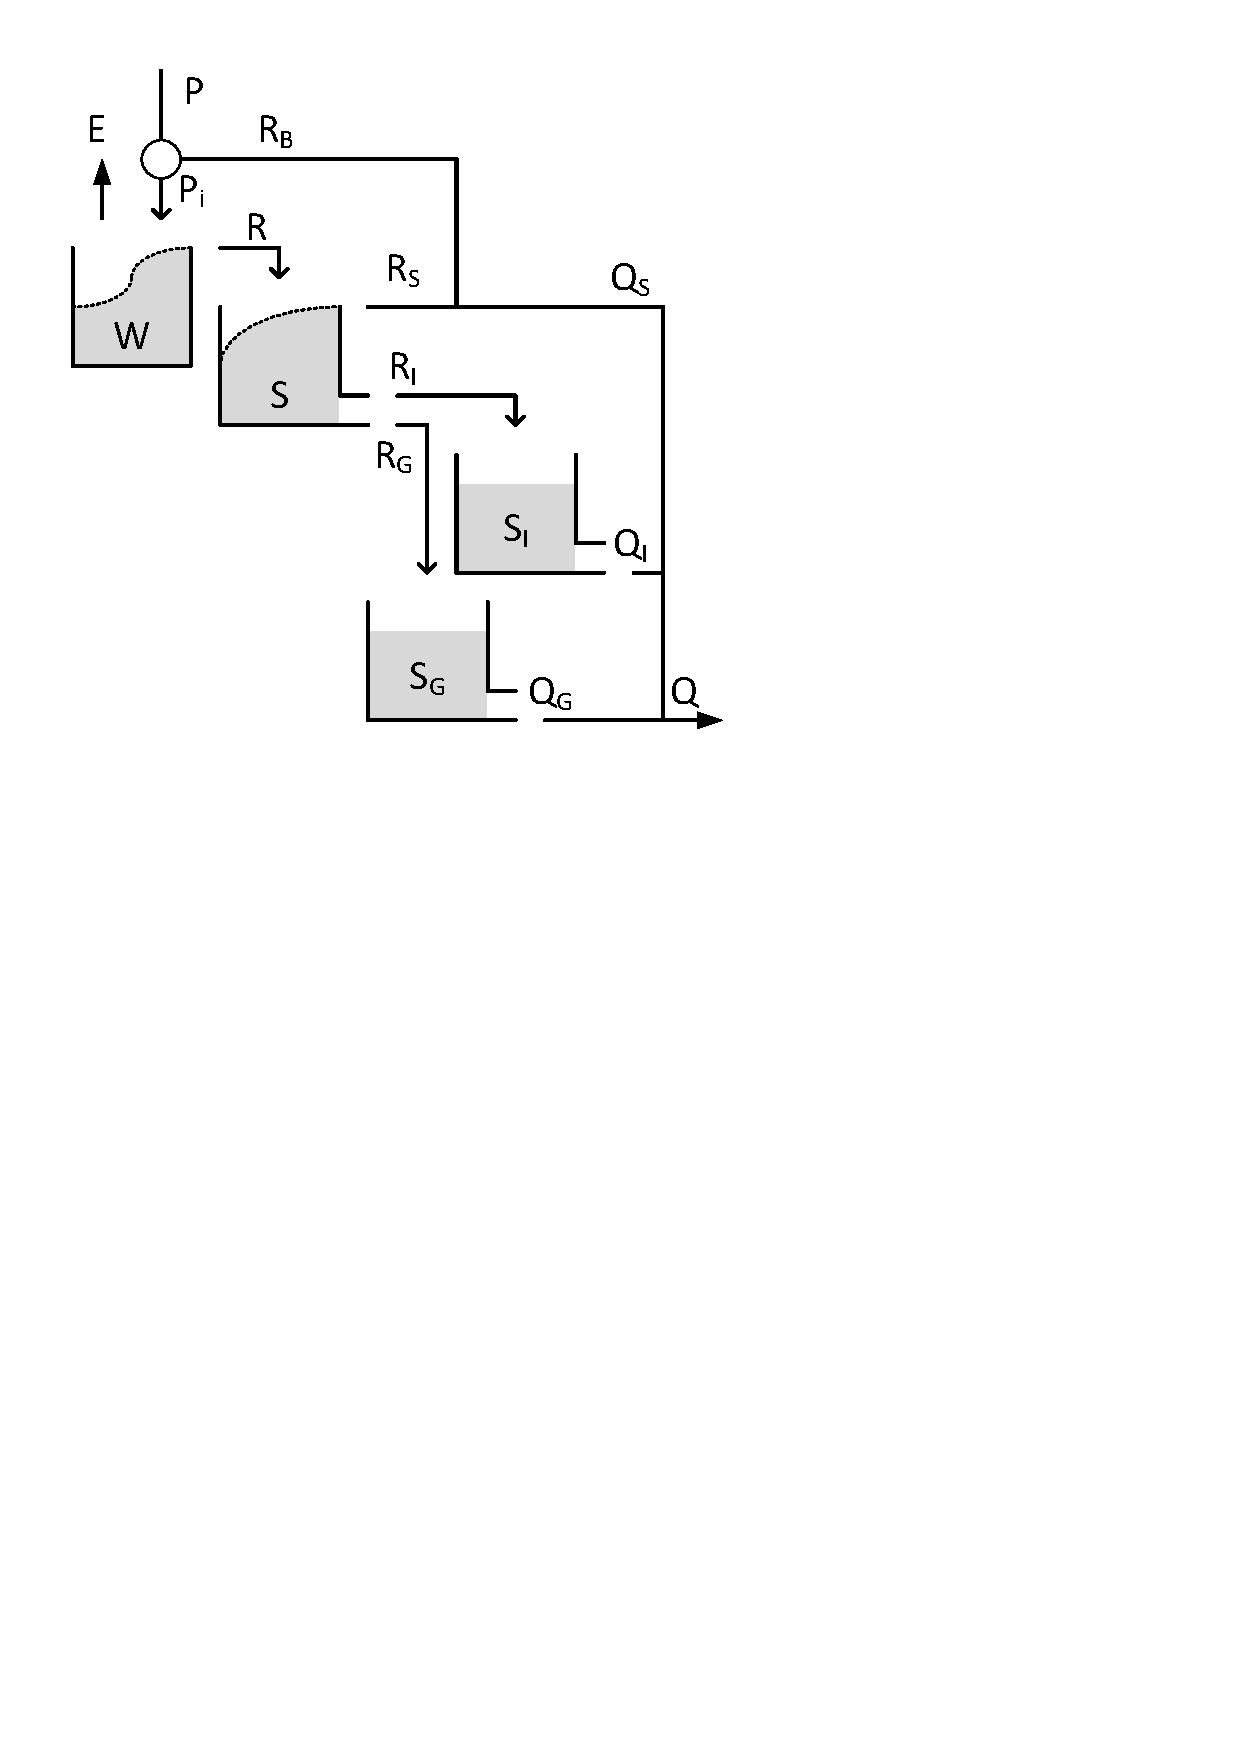
\includegraphics[trim=1cm 17cm 7cm 1cm,width=7cm,keepaspectratio]{./files/28_schematic.pdf}
\caption{Structure of the Xinanjiang model} \label{fig:28_schematic}
\end{wrapfigure}

\begin{align}
	\frac{dW}{dt} &= P_i-E-R \\
	P_i &= (1-A_{im})*P \\
	R &= 
	\begin{cases}
		P_i * \left[(0.5-a)^{1-b}\left(\frac{W}{W_{max}}\right)^b\right] , & \text{if } \frac{W}{W_{max}} \leq 0.5-a \\
		P_i * \left[1-(0.5+a)^{1-b}\left(1-\frac{W}{W_{max}}\right)^b\right] , & \text{otherwise}
	\end{cases} \\
	E &= \begin{cases}
		E_p , & \text{if } W > LM \\
		\frac{W}{LM}E_p , & \text{if } c*LM \geq W \leq LM \\
		c*E_p , & \text{otherwise}
	\end{cases}
\end{align}

} % end of wrapfigure fix
\vspace{2cm}
Where $W$ [mm] is the current tension water storage, refilled by a infiltration $P_i$ $[mm/d]$ and drained by evaporation $E$ $[mm/d]$ and runoff $R$ $[mm/d]$.
$P_i$ is the fraction of precipitation $P$ $[mm/d]$ that does not fall on impervious area $A_{im}$ [-].
Runoff generation $R$ uses a double parabolic curve to determine the fraction of catchment area that is at full tension storage and thus can contribute to runoff generation. 
This curve relies on shape parameters $a$ [-] and $b$ [-], and maximum tension water storage $W_{max}$ [mm].
Evaporation rate $E$ declines as tension water storage decreases.
Evaporation occurs at the potential rate $E_p$ $[mm/d]$ if storage $W$ is above threshold $LM$ [mm], and reduces linearly below that up to a second threshold $c*LM$ [-]*[mm].
Below this threshold evaporation occurs at a constant rate $c*E_p$.

\begin{align}
	\frac{dS}{dt} &= R-R_S-R_I-R_G\\
	R_S &= R*\left(1-\left(1-\frac{S}{S_{max}}\right)^{Ex}\right) \\
	R_I  &= k_I * S * \left(1-\left(1-\frac{S}{S_{max}}\right)^{Ex}\right)\\
	R_G  &= k_G * S * \left(1-\left(1-\frac{S}{S_{max}}\right)^{Ex}\right)
\end{align}

Where $S$ [mm] is the current storage of free water, refilled by runoff $R$ from filled tension water areas, and drained by surface runoff $R_S$ [mm/d], interflow $R_I$ [mm/d] and baseflow $R_G$ [mm/d].
All runoff components rely on a parabolic equation to simulate variable contributing areas of the catchment, dependent on maximum free water storage $S_{max}$ [mm] and shape parameter $Ex$ [-]. 
$R_I$ also uses a time coeficient $k_I$ $[d^{-1}]$.
$R_G$ uses a time coeficient $k_G$ $[d^{-1}]$.

\begin{align}
	\frac{dS_I}{dt} &= R_{I} - Q_I\\
	Q_I &= c_I*S_I 
\end{align}

Where $S_I$ [mm] is the current storage in the interflow routing reservoir, filled by interflow from free water $R_I$ and drained by delayed interflow $Q_I$ $[mm/d]$.
$Q_I$ uses a time coefficient $c_I$ $[d^{-1}]$.

\begin{align}
	\frac{dS_G}{dt} &= R_{G} - Q_G\\
	Q_G &= c_G*S_G
\end{align}

Where $S_G$ [mm] is the current storage in the baseflow routing reservoir, filled by baseflow from free water $R_G$ and drained by delayed baseflow $Q_G$ $[mm/d]$.
$Q_G$ uses a time coefficient $c_G$ $[d^{-1}]$.
Total flow depends on four separate runoff components:

\begin{align}
	Q_t &= Q_S + Q_I + Q_G \\
	Q_S &= R_S + R_B \\
	R_B &= A_{im}*P
\end{align}

Where $R_B$ [mm/d] is direct rainoff generated by precipitation $P$ [mm/d] on the fraction impervious area $A_{im}$ [-].

\subsubsection{Parameter overview}
% Table generated by Excel2LaTeX from sheet 'Sheet1'
\begin{table}[htbp]
  \centering
    \begin{tabular}{lll}
    \toprule
    Parameter & Unit  & Description \\
    \midrule
    $A_{im}$ & $-$   & Fraction impervious area \\
    $a$   & $-$   & Contributing area curve inflection point \\
    $b$   & $-$   & Contributing area curve shape parameter \\
    $W_{max}$ & $mm$  & Maximum tension water storage \\
    $LM$  & $mm$  & Threshold for evaporation behaviour change \\
    $c$   & $-$   & Threshold and evaporation reduction factor \\
    $S_{max}$ & $mm$  & Maximum free water storage \\
    $Ex$  & $-$   & Contributing area curve shape parameter \\
    $k_I$ & $d^{-1}$ & Runoff coefficient \\
    $k_G$ & $d^{-1}$ & Runoff coefficient \\
    $c_I$ & $d^{-1}$ & Runoff coefficient \\
    $c_G$ & $d^{-1}$ & Runoff coefficient \\
    \bottomrule
    \end{tabular}%
  \label{tab:addlabel}%
\end{table}%
